\newpage
\section{Results}

\subsection{4 Alternative forced choice task}

The fitted logistic functions returned four perception thresholds that where not covered by our stimulus range. Consequently, we excluded these subjects from subsequent analyses. The excluded fits are indicated as gray lines in figure \ref{fig:4afc_psychofit}. The perception thresholds inferred from the fitted sigmoids ranged from 30 ms to 90 ms. The thresholds compared for the two conditions of differing spatial frequencies were not significant but showed a light trend (Wilcoxon, Z = 1.5, p = 0.06) see also figure \ref{fig:4afc_psychofit}, Right. Except for a one individual, all subjects showed the trend that higher spatial frequencies resulted in a higher detection threshold.

Because our data indicates that smaller spatial frequencies are harder to perceive, we used the same two stimulus levels in the comparative visual search task to manipulate the detectability of the stimuli.

\begin{figure}[H]
    \centering
    \includesvg[width=\textwidth]{Figures/4afc_psychofit.svg}
    \caption[4AFC psychofit]{Fitted data from the 4AFC task (\textbf{Left} and \textbf{Middle}). Stimulus duration on the x-axis and probability of correct answer on the y-axis. The detection threshold is marked with a point and a line on the x-axis. Curves are colorcoded so that each color corresponds to one subject in each plot. Gray curves are excluded from our analysis therefore don't appear in the \textbf{right} plot. \textbf{Right}: Detection threshold for the two spatial frequencies for each subjects. Each color corresponds with one subject.}
    \label{fig:4afc_psychofit}
\end{figure}

\subsection{Comparative visual search task}
One subject had to be excluded due to too many trials without switches ($>5$). The subjects were mostly able to maintain performance regarding trial duration and error rate throughout the experiment and also did not change their number of switches per trial with experiment progress (see \ref{fig:trial_stability}). 

\begin{figure}[H]
    \centering
    \includesvg[width=\textwidth]{Figures/trial_stability.svg}
    \caption[Mean performance over trials]{Mean performance over trials for number of switches, trial duration and correct answers. Black line represents the mean of all subjects, which are shown as gray lines. One subject took a lot more time in some trials, another subject partly performed substantially below average in percent correct answers. Overall, trial number did not influence performance or strategy.}
    \label{fig:trial_stability}
\end{figure}

\subsubsection{Population level effects}

When comparing the results between different stimulus conditions, also the median error rate stayed constant throughout conditions (see \ref{fig:boxplots1}), as well as the number of switches (\ref{fig:boxplots2}). However, the response time and, as the number of switches did not change significantly (W = 0, $p<0.05$), the processing time increased significantly in the high spatial frequency trials as compared to the trials with low spatial frequency Gabor patches (W = 0, $p<0.05$). Note that the outlier (VP6) in response time and thus processing time stretches the scale quite substantially, so no uniform distribution can be assumed anymore. 

\begin{figure}[H]
    \centering
    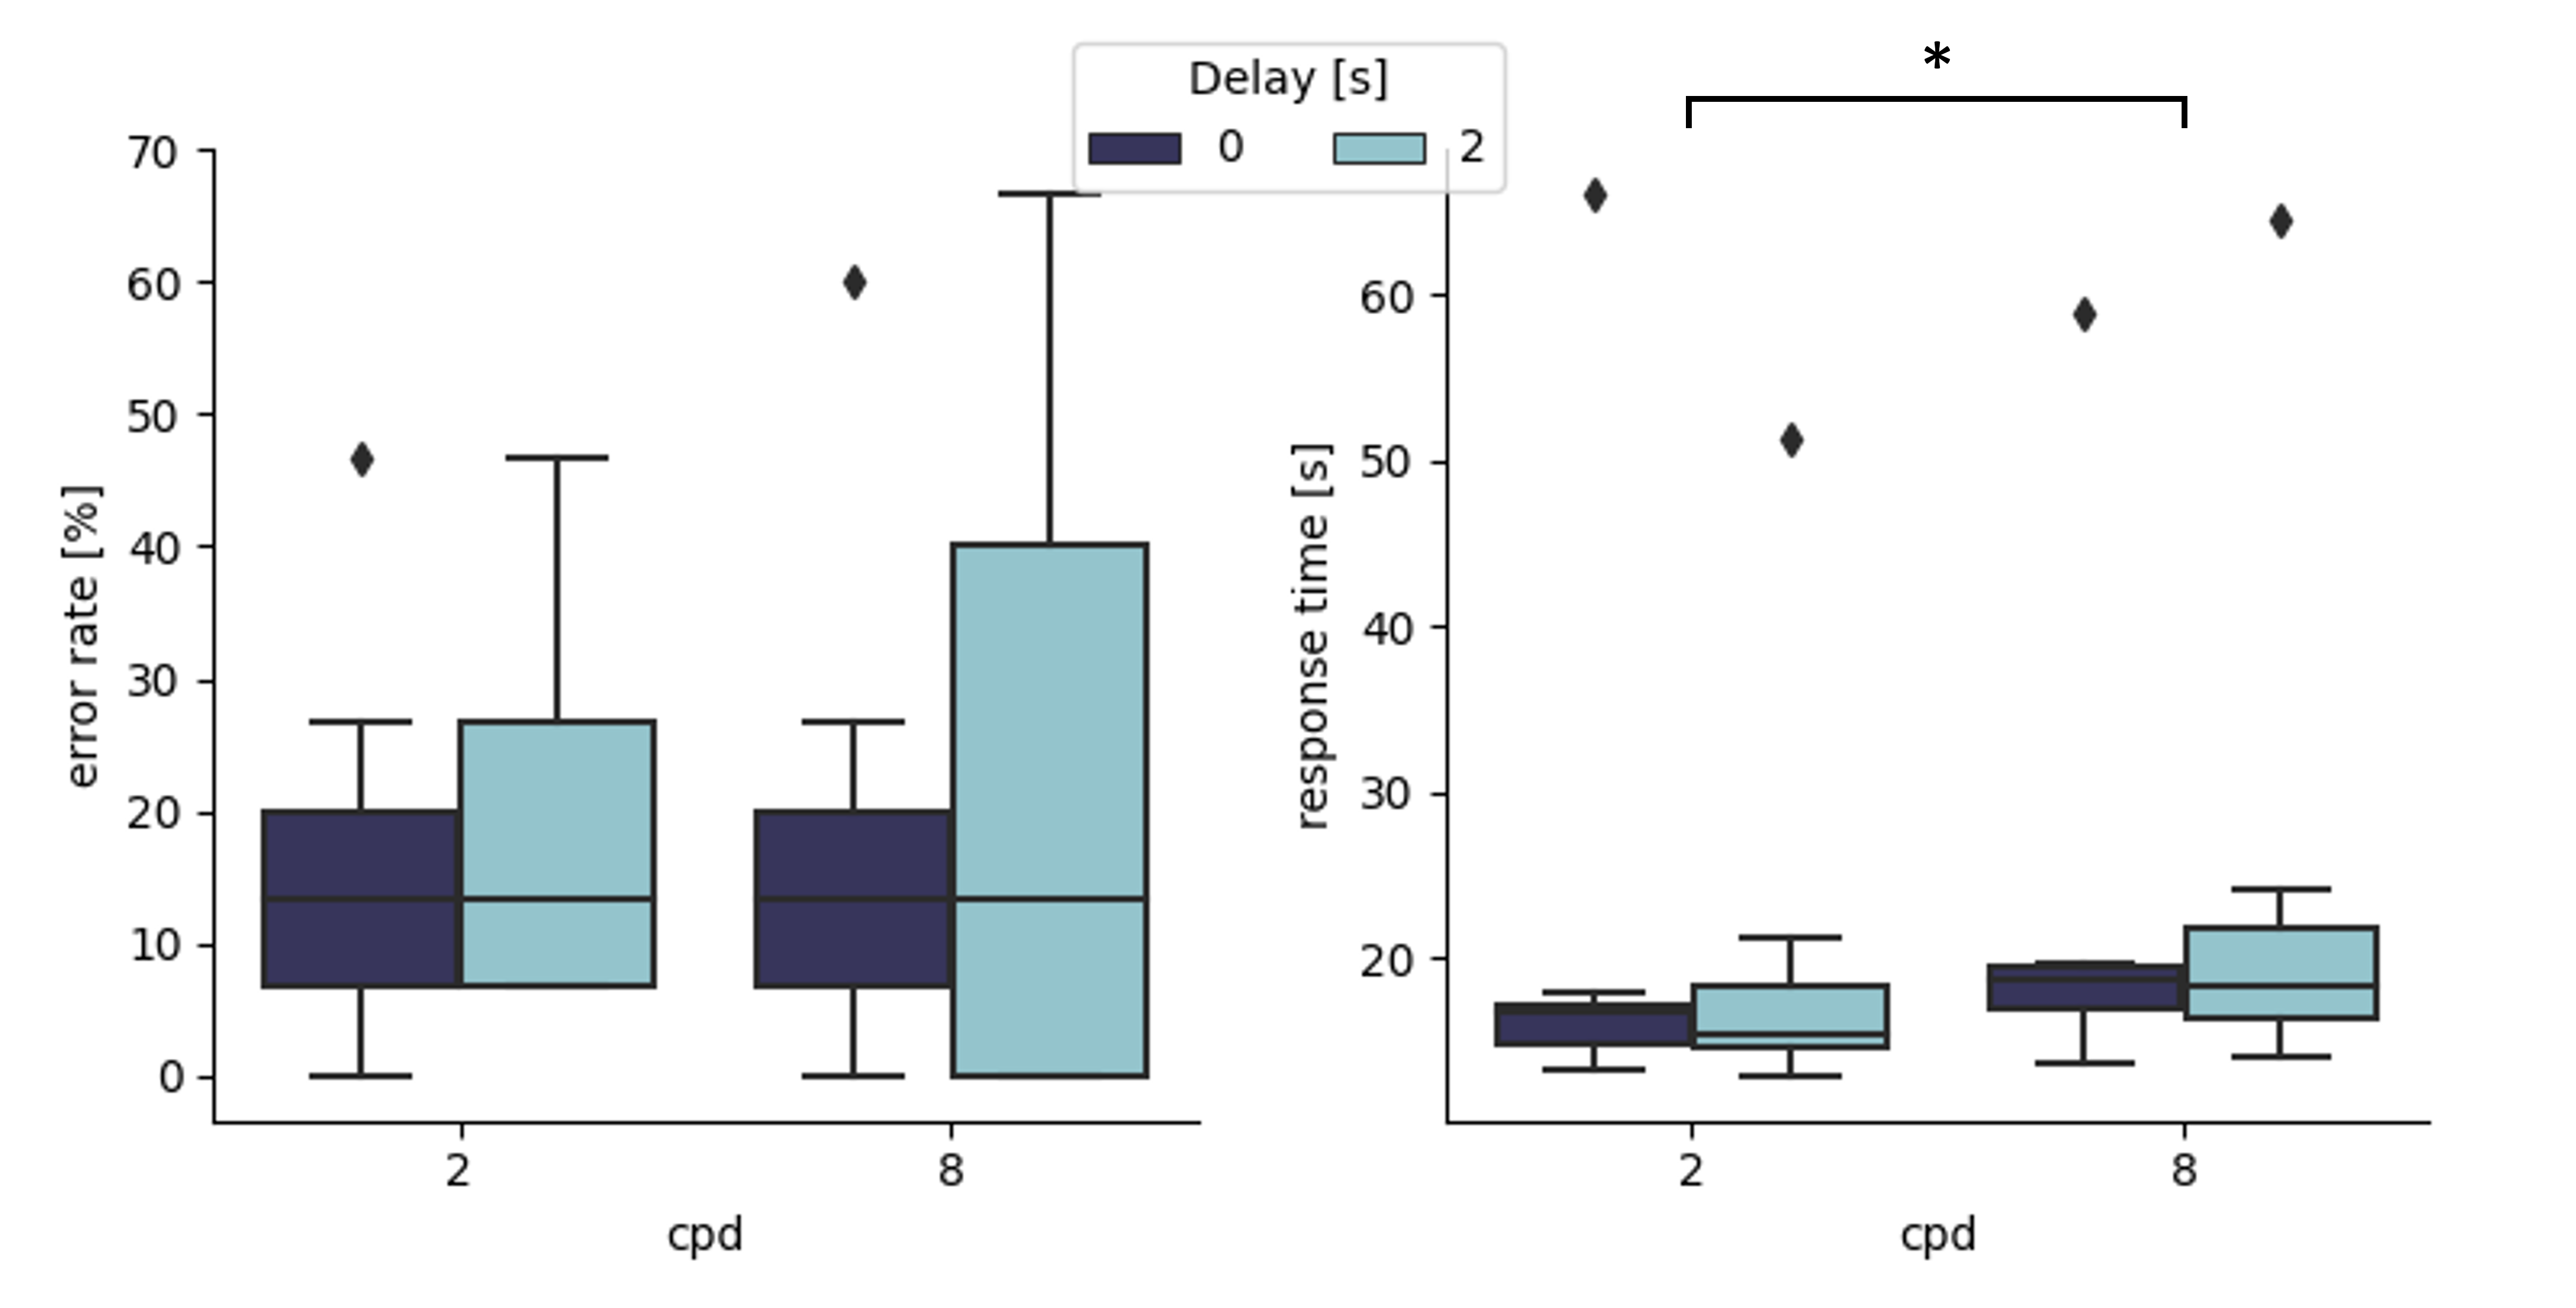
\includegraphics[width=\textwidth]{Figures/box_plots_err+resp_protocol.png}
    \caption[Error rate and response time]{Error rate and response time for different stimulus conditions. Boxplots are shown for 2 and 8 cycles per degrees and colour-coded for 0 and 2 seconds delay respectively. A significant difference can only be found between 2 and 8 cycles per degree (W = 0, $p<0.05$) for response times.}
    \label{fig:boxplots1}
\end{figure}

\begin{figure}[H]
    \centering
    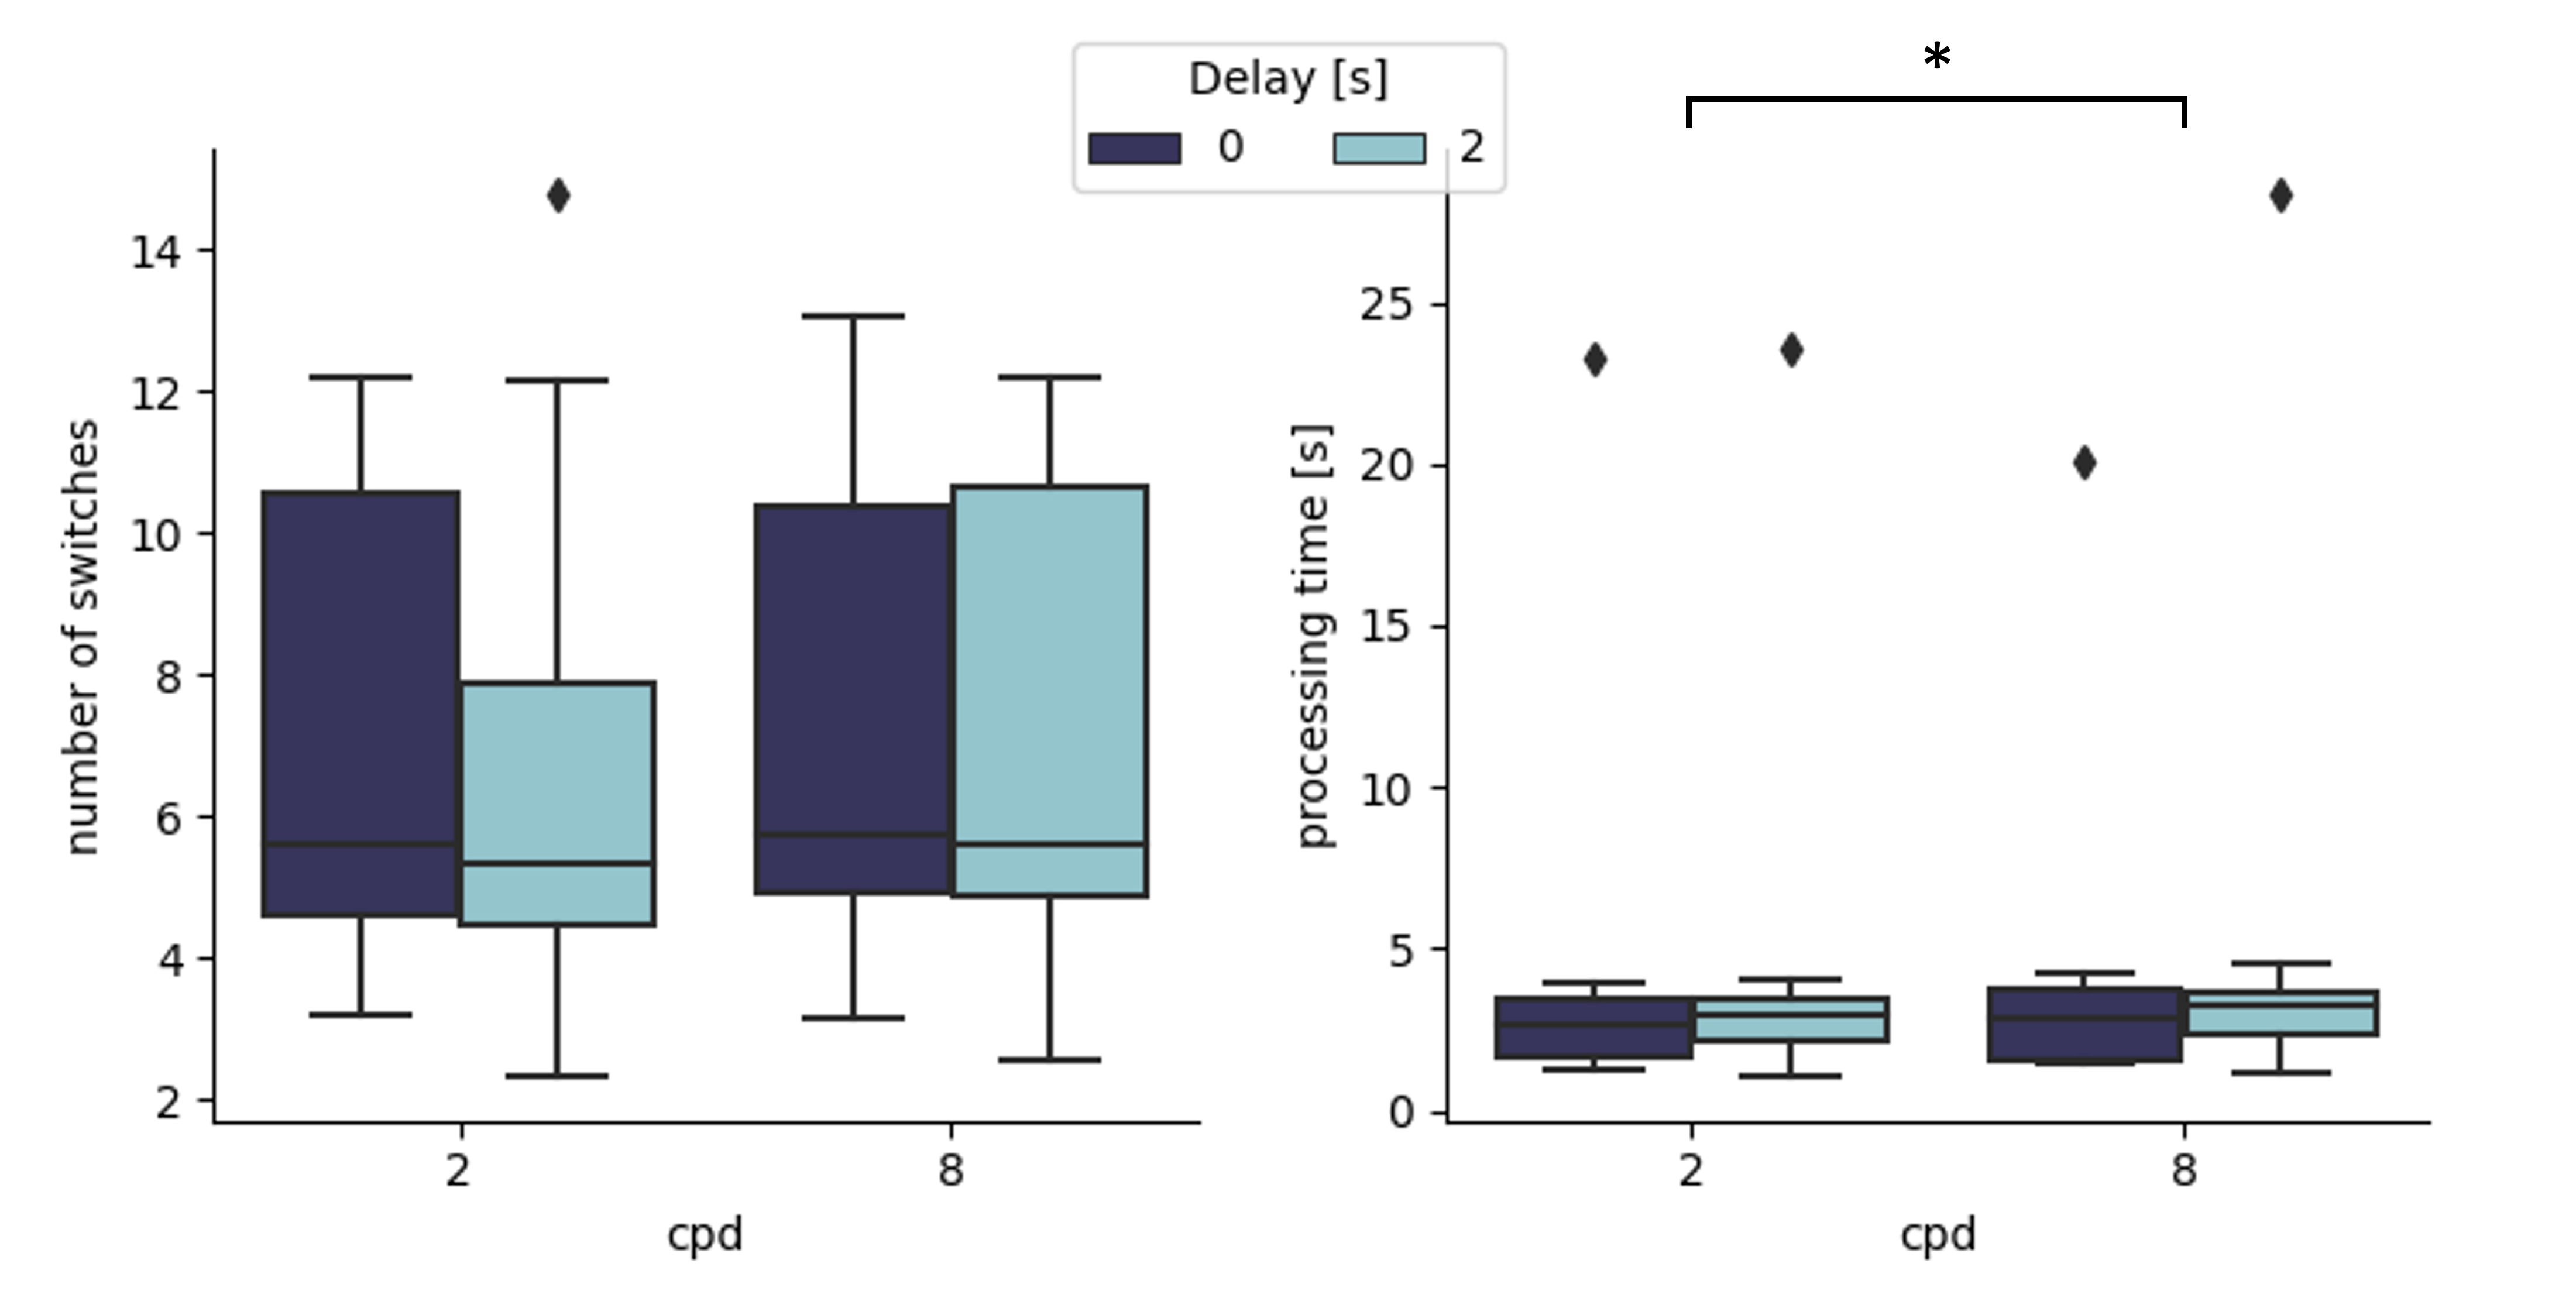
\includegraphics[width=\textwidth]{Figures/box_plots_shifts+proc_protocol.png}
    \caption[Switches and processing time]{Number of switches and processing time for different stimulus conditions. Boxplots are shown for 2 and 8 cycles per degrees and colour-coded for 0 and 2 seconds delay respectively. A significant difference can only be found between 2 and 8 cycles per degree (W = 0, $p<0.05$) for processing times.}
    \label{fig:boxplots2}
\end{figure}

\newpage
\subsubsection{Individual level effects}

To get an insight into the distribution of individual strategies, we plotted the strategy spaces spanned by the processing time and the number of gaze shifts (\ref{fig:cvs_powerfit}). Each individual is represented by its mean and SEM across all categories for both variables. The majority of our subjects clustered in the bottom right, indicating acquisition strategists, whereas a single individual leaned strongly towards memorization.

\begin{figure}[h]
    \centering
    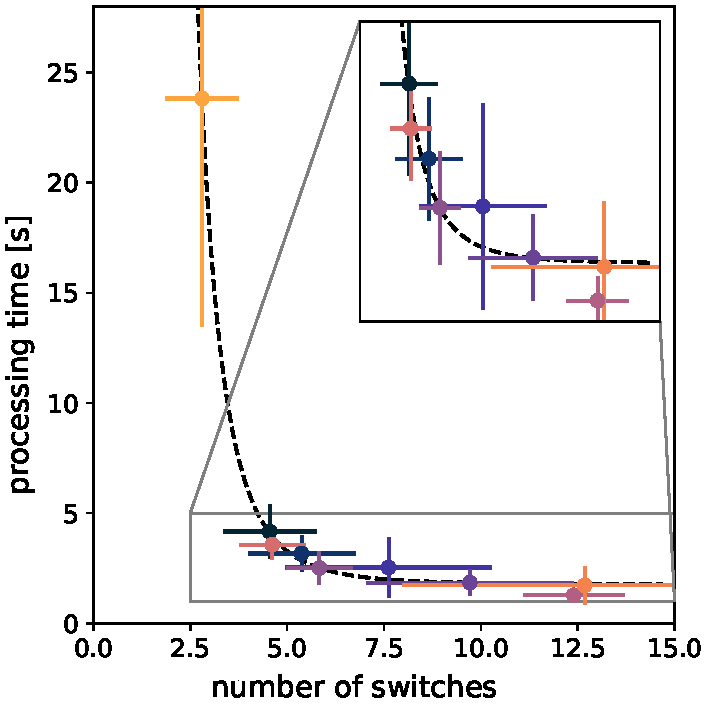
\includegraphics[width=0.7\textwidth]{Figures/cvs_all_powerfit.pdf} 
    \caption[Strategy space]{Strategy space for all included individuals across all stimulus categories. Colors represent individuals. The points indicate the mean of the respective individual on the respective dimension. The error bars show the standard error. The dashed line shows a powerlaw function fitted to the means. The inset shows the fit in detail for the cluster in the lower right to better asses the powerlaw fit in that region. The outlier (yellow) is included since it did not strongly affected the fit.}
    \label{fig:cvs_powerfit}
\end{figure}

Increasing the difficulty of perception, i.e. increasing the cycles per degree in the 8 cpd condition lead to a consistent change: Individuals increased the amount in which they used their previously observed strategy. That is, individuals that worked with memorization increased their memorization time, while individuals that worked with acquisition increased their number of gaze shifts (\ref{fig:cvs_powerfit_cpd}). 

\begin{figure}[h]
    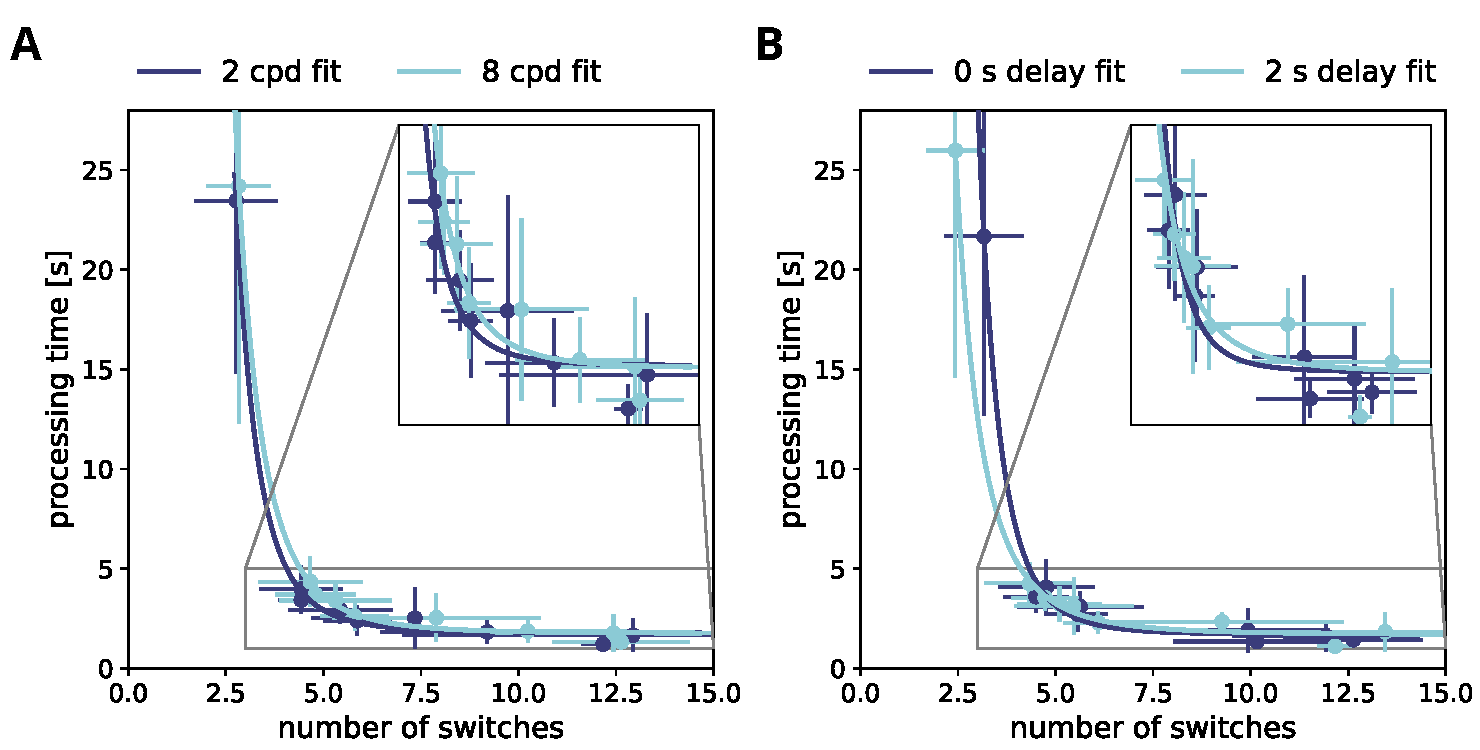
\includegraphics[width=\textwidth]{Figures/comb.pdf}
    \caption[CVS powerfit cpd]{Strategy space separated (a) by cycles per degree conditions (two shades of blue) and (b) by delay. The increase in cycles per degree move the individual mean up the axis it utilizes the most: Points in the bottom right move more towards the bottom right. Points in the center move along the diagonal. Increasing the delay shifted the strategy of all individuals towards memorization.}
    \label{fig:cvs_powerfit_cpd}
\end{figure}

The strategy index reflected the same pattern that was observable on the strategy space: Most subjects clustered on the acquisition end of the spectrum and a single outlier strongly leans towards memorization.

\begin{figure}[H]
    \centering
    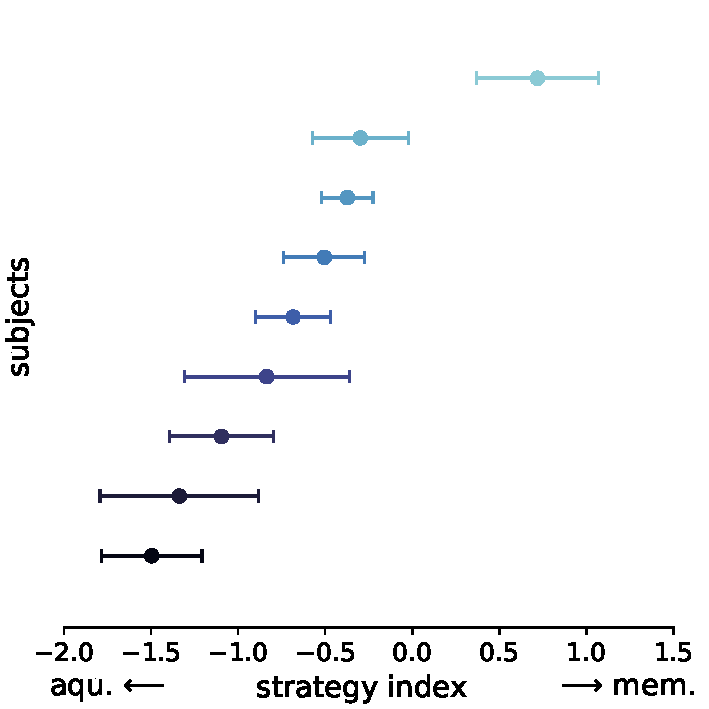
\includegraphics[width=0.7\textwidth]{Figures/stratidx.pdf}
    \caption[Strategy index overview]{Strategy index colored by subject ID grouped across all stimulus regimes. The distribution of subjects along the strategy index resembles the distribution observable in the two dimensional strategy space in figure \ref{fig:cvs_powerfit}.}
    \label{fig:strategy_index}
\end{figure}

The strategy indices separated by delay and cycles per degree condition respectively (\ref{fig:strategy_index_cpd} show the same pattern already visible in the strategy space.

\begin{figure}[H]
    \centering
    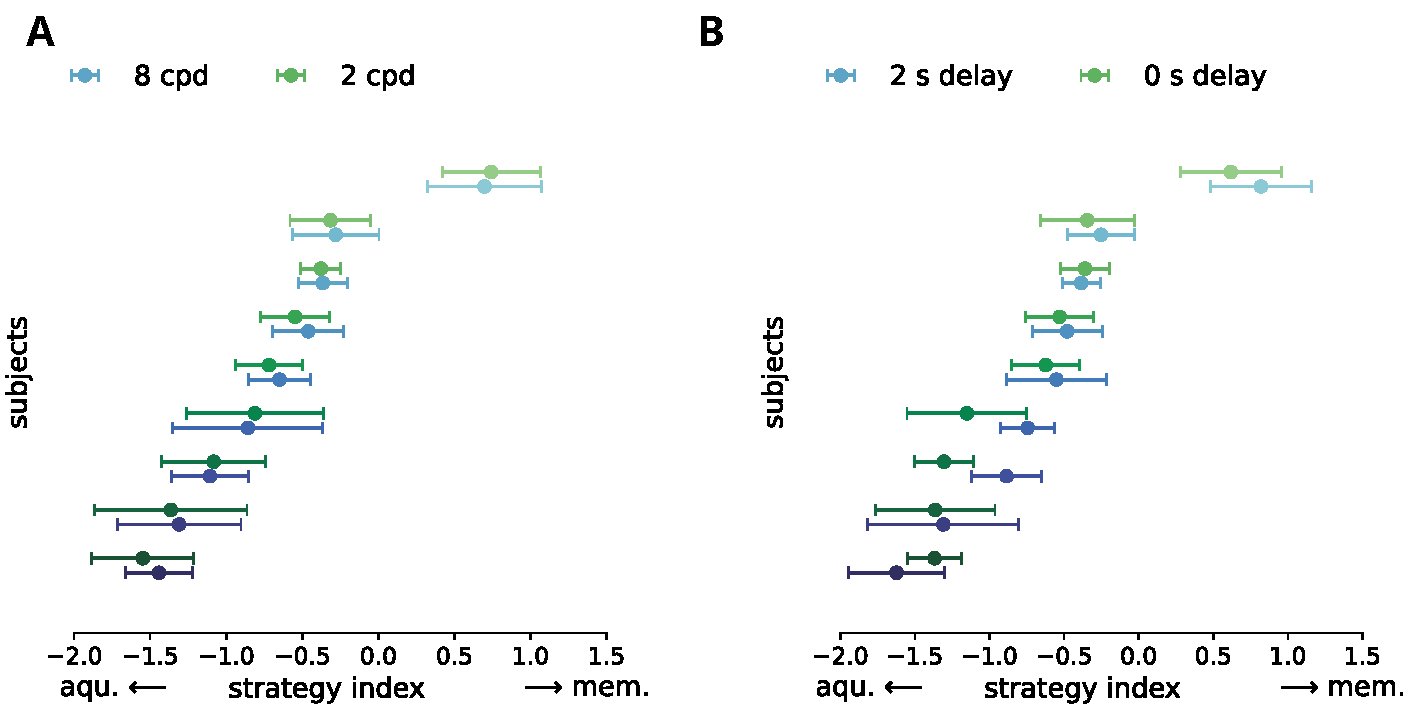
\includegraphics[width=\textwidth]{Figures/stratidx_cpd4.pdf}
    \caption[Strategy index by spatial frequency and delay]{Strategy indices separated by the two spatial frequencies (a) and the two delay conditions (b). In both cases, the same pattern observed in the strategy space can be observed here as well: Changes in the difficulty of perception (a) seem to shift acquisition strategists more towards acquisition, whereas memorization strategists are shifted more towards memorization. Raising the acquisition costs seem to shift all individuals towards increased memorization.}
    \label{fig:strategy_index_cpd}
\end{figure}

If a subject had difficulties perceiving the stimulus, i.e. had a higher detection threshold in the 4AFC task, we expected them to lean more towards a memorization rather than aquisition strategy. 
To relate the individuals strategy to the detection threshold, we computed a linear regression of the detection threshold and the strategy index but did not find a relationship between the two in our dataset.

\vspace{5mm}
\subsection{Contrast sensitivity}

The fitted logistic functions returned perception thresholds ranging from 0.017 to 0.019 Michelson contrast for the lower spatial frequency. The perception threshold for Michelson contrast for the higher spatial frequency of 20\,cpd is outside the range of presented contrasts for all three subjects. All three subjects reported that they didn't perceive the stimulus  for any contrast in the 20\, cpd condition. The mean perception threshold of 0.0173 in the condition with the lower spatial frequency is lower than the mean perception threshold of $>$ 0.64 in the high spatial frequency condition. 

\begin{figure}[H]
    \centering
    \includesvg[width=\textwidth]{Figures/contrast_sensitivity.svg}
    \caption[Contrast sensitivity]{Psychometric function for contrast sensitivity for all three subjects. On the Y-axis is the proportion of correct answers, on the X-axis is the range of presented Michelson contrasts. Colors are matched to the subjects in both plots. \textbf{Left:} Curves for a low spatial frequency (10\,cpd) \textbf{Right:} Curves for a high spatial frequency (20\,cpd)}
    \label{fig:contrast_sensitivity}
\end{figure}

